\documentclass[9pt]{beamer}
% Created By Gouthaman KG

% Use roboto Font (recommended)
\usepackage{physics,commath}
\usepackage{amsmath,amsthm,amsfonts,amssymb,bm}
\usepackage{graphicx,subfigure}

\usepackage[sfdefault]{roboto}
\usepackage[utf8]{inputenc}
\usepackage[T1]{fontenc}


% Define where theme files are located. ('/styles')
\usepackage{styles/fluxmacros}
\usefolder{styles}
% Use Flux theme v0.1 beta
% Available style: asphalt, blue, red, green, gray
\usetheme[style=asphalt]{flux}


% Extra packages for the demo:
\usepackage{booktabs}
\usepackage{colortbl}
\usepackage{ragged2e}
\usepackage{schemabloc}
\usepackage{hyperref}
\usebackgroundtemplate{

\includegraphics[width=\paperwidth,height=\paperheight]{assets/background.jpg}}
%change this to your preferred background for the presentation.

% Informations
\title{3-D mass map reconstruction}
\subtitle{Method and Plane in S19A}

\author{Xiangchong Li\\
Colaborators:\\
Naoki Yoshida, Masamune Oguri\\
Shiro Ikeda, Wentao Luo
}
%\institute{The University of Tokyo}
\titlegraphic{assets/gkg.png}
%change this to your preferred logo or image(the image is located
%on the top right corner).
%~~~~~~~~~~~~~~~~~~~~~~~~~~~~~~~~~~~~~~~~~~~~~~~~~~~~~~~~~~~~~~~~~~~~~~~~~~~~~~

\begin{document}

% Generate title page
\titlepage


\section{3-D Mass Map Construction}
\newcommand \figPathM{/home/xiangchong/.local/code/massMap_Private/doc/paper_ms_method_HSCY1/}
\newcommand \figPathMF{/home/xiangchong/.local/code/massMap_Private/doc/fig/}
\newcommand{\argmax}{\mathop{\rm arg~max}\limits}
\newcommand{\argmin}{\mathop{\rm arg~min}\limits}

\subsection{Model Dictionary and Regularization}
\begin{frame}{Goal}
\begin{equation} \notag
    \gamma=\mathbf{T} \delta+\rm{noise},
\end{equation}
where $\mathbf{T}$ includes both physical signal and systematics
\begin{columns}[t]
\begin{column}{0.5\textwidth}
{\color{blue}\rule{\linewidth}{4pt}
Physical Signal}\\
\begin{equation}\notag
\kappa(\vec{\theta},z_s)=\frac{3H_0^2\Omega_M}{2 c^2} \int_0^{\chi_s} d\chi_l \frac{\chi_l \chi_{sl}}{\chi_s}
\frac{\delta(\vec{\theta},z_l)}{a(\chi_l)},
\end{equation}
\begin{equation}\notag
\gamma_L(\vec{\theta},z_s) = \int  d^2 \theta' D(\vec{\theta}-\vec{\theta'}) \kappa(\vec{\theta'},z_s),
\end{equation}
where
\begin{equation}\notag
D(\vec{\theta})=-\frac{1}{\pi}(\theta_1-i\theta_2)^{-2}.
\end{equation}
\end{column}
\hfill
\begin{column}{0.5\textwidth}
{\color{red}\rule{\linewidth}{4pt}
Systematics}
\begin{itemize}
    \item photo-$z$ uncertainty;
    \item Masking;
    \item Smoothing in transverse plane;
    \item Pixelization.
\end{itemize}
\end{column}
\end{columns}
\alert{Goal: Inverse the matrix $\mathbf{T}$ and estimate $\delta(\vec{\theta},z_l)$.}
\begin{equation} \notag
\hat{\delta}=\argmin_{x} \left\{ \frac{1}{2}\norm{\Sigma^{-\frac{1}{2}}(\gamma-
\mathbf{T} \delta)}_2^2\right\}.
\end{equation}
\end{frame}

\begin{frame}{Prior Information}
Since the $3$-D inversion problem is an \alert{ill-posed problem}, we have to add \alert{prior information}.
\begin{columns}[t]
\begin{column}{0.5\textwidth}
\begin{alertblock}{Model Dictionary}
\begin{equation} \notag
\delta(\vec{\theta},z)=\Sigma_{i} \Phi_i(\vec{\theta},z) x_i,
\end{equation}
where $\Phi_i$ is the model basis, and $x_i$ is the projected modes.
e.g.,
\begin{enumerate}
    \item Point Mass;
    \item Fourier Space (sine, cosine);
    \item Starlets.
\end{enumerate}
\end{alertblock}
\end{column}

\begin{column}{0.5\textwidth}
\begin{alertblock}{Regularization}
\begin{equation} \notag
\hat{x}=\argmin_{x} \left\{ \frac{1}{2}\norm{\Sigma^{-\frac{1}{2}}(\gamma-
\mathbf{T} \Phi x)}_2^2+ \lambda \norm{x}_p^p \right\},
\end{equation}
\begin{equation}\notag
\norm{x}_p^p=(\sum_{i} |x|^p_i).
\end{equation}
e.g.,
\begin{enumerate}
    \item $p=2$, \alert{Ridge regression} (Wiener Filter);
    \item $p=1$, \alert{Lasso} (Sparse);
    \item $p=0$, \alert{Best subset} (sparsest but NP hard).
\end{enumerate}
\end{alertblock}
\end{column}
\end{columns}
Choose a \alert{model dictionary} and a \alert{regularization
(Prior distribution of $x$)}.
\end{frame}


\subsection{Line of Sight Smearing}
% \begin{frame}{Line of sight smearing}
% \begin{figure}
% \includegraphics[height=0.6 \textwidth]{\figPathMF Richard_Massey_HST.png}
% \end{figure}
% Richard Massey (HST)
% \end{frame}

\begin{frame}{Wiener Filter in S16A}
\begin{figure}
\includegraphics[height=0.6 \textwidth]{\figPathMF Masamune_Oguri_HSC.png}
\end{figure}
Masamune Oguri, 2018 (HSC), Wiener Filter
\end{frame}

\begin{frame}{NFW Model dictionary}
\begin{columns}
\begin{column}{0.4\textwidth}
\begin{figure}
\includegraphics[width=1.0\textwidth]{\figPathM nfwlet-atom-1D.pdf}
\end{figure}
\begin{itemize}
    \item pixel size:  $1$ arcmin;
    \item Gaussian Smoothing: $1.5$ arcmin;
    \item Three NFW scales: $0.12$, $0.24$, and $0.36~h^{-1}$  Mpc.
\end{itemize}
\end{column}
\begin{column}{0.6\textwidth}
\begin{alertblock}{NFW Atoms}
On the transverse Plane
\begin{eqnarray}\notag
\phi_\alpha(\vec{r}) =&\frac{f }{2 \pi \theta_\alpha^2 }
F(|\vec{\theta}|/\theta_\alpha) \delta_D(z),\\
&  (\alpha=1..N)\notag
\end{eqnarray}
\begin{equation}\notag
F(x)=
\begin{cases}
-\frac{\sqrt{c^2-x^2}}{(1-x^2)(1+c)} + \frac{\rm{arccosh}
\left(\frac{x^2+c}{x(1+c)}\right)}{(1-x^2)^{3/2}}  & (x<1),\\
\frac{\sqrt{c^2-1}}{3(1+c)} (1+\frac{1}{c+1}) & (x=1),\\
-\frac{\sqrt{c^2-x^2}}{(1-x^2)(1+c)} +
\frac{\arccos\left(\frac{x^2+c}{x(1+c)}\right)}{(x^2-1)^{3/2}} & (1<x\leq c),\\
0& (x>c).
\end{cases}
\end{equation}
Takada \& Jain (2003)
\end{alertblock}
\end{column}
\end{columns}
\end{frame}

\begin{frame}{Adaptive Lasso (regularization/Prior on $x$)}
\alert{Approximation to $l^0$ regularization with two steps of
$l^1$ lasso estimation}\\
Zou (2007)
\begin{alertblock}{first step: lasso}
\begin{equation}\notag
\hat{x}=\argmin_{x} \left\{ \frac{1}{2} \norm{\Sigma^{-\frac{1}{2}}(\gamma-\mathbf{A}x)}^2_2 +
\lambda \norm{x}^1_1\right\}.
\end{equation}
\end{alertblock}
\begin{equation}
\hat{w}= \frac{1}{\abs{\hat{x'}^{\rm{lasso}}}^\tau},
\end{equation}
hyper-parameter: $\tau=2$.
\begin{alertblock}{second step: weighted lasso}
\begin{equation}\notag
\hat{x}=\argmin_{x} \left\{ \frac{1}{2} \norm{\Sigma^{-\frac{1}{2}}(\gamma-\mathbf{A}x)}^2_2 +
\hat{w}\lambda_{\rm{ada}} \norm{x}^1_1\right\}.
\end{equation}
\end{alertblock}
\end{frame}


\begin{frame}{Results for Noiseless Simulation}
\begin{itemize}
    \item One halo in $1\deg^2$
    \item HSC (s16) number densitty;
    \item HSC (s16) redshifts(best estimation);
    \item No noise; no photo-$z$ uncertainty.
\end{itemize}
\begin{figure}
\centering
\includegraphics[width=1.0\textwidth]{\figPathMF results_noiseless.png}
\end{figure}
\end{frame}


\begin{frame}{Correlated Lensing Kernels}
\begin{figure}
 \centering
 \includegraphics[width=1.0\textwidth]{\figPathM lensing_kernel.pdf}
\end{figure}
\alert{The lensing kernels for two neighbouring lens redshift bins
are too correlated (The shapes of them are similar). Therefore, it
is difficult to distinguish in which bins the mass is actually
located.}
\end{frame}


\begin{frame}{Results on simulations}
\begin{itemize}
    \item One halo in $1\deg^2$
    \item HSC (s16) number densitty;
    \item HSC (s16) redshifts(best estimation);
    \item HSC (s16) shape noise; HSC photo-$z$ uncertainty.
\end{itemize}
\begin{figure}
\centering
\includegraphics[width=1.0\textwidth]{\figPathMF results_noisy.png}
\end{figure}
\end{frame}

\begin{frame}{Peak Histogram}
Pure Noise field:
\begin{itemize}
    \item $1000$ pure noise realizations with HSC shape noise and photoz
    uncertainty.
\end{itemize}
Halos:
\begin{itemize}
    \item $81$ halos with different mass and redshift;
    \item Each halo has $100$ noise realizations.
\end{itemize}
\begin{figure}
\centering
\includegraphics[width=1.0\textwidth]{\figPathM peak_histograms_NFW.pdf}
\end{figure}
\end{frame}

\begin{frame}{Detections for difference thresholds}
    \begin{itemize}
        \item $\lambda=5.0$
    \end{itemize}
\begin{figure}
\centering
\includegraphics[width=1.0\textwidth]{\figPathM detfalse_threshold_NFW_lbd50.pdf}
\end{figure}
\end{frame}
\begin{frame}{Redshift estimation}
    We simulation halos with different mass at different redshift; each halo with $100$ noise realizations. The following figures show the \alert{offsets} of detected peaks from the input positions.
\begin{figure}
\centering
\includegraphics[width=1.0\textwidth]{\figPathM peak_scatters_NFW_lbd35.pdf}
\end{figure}
\end{frame}





\begin{frame}{Preliminary run on $1$ deg$^2$ region of XMM}
\begin{itemize}
    \item S19A data
    \item corrected for additive bias
    \item set multiplicative bias to zero
\end{itemize}
\begin{figure}
\centering
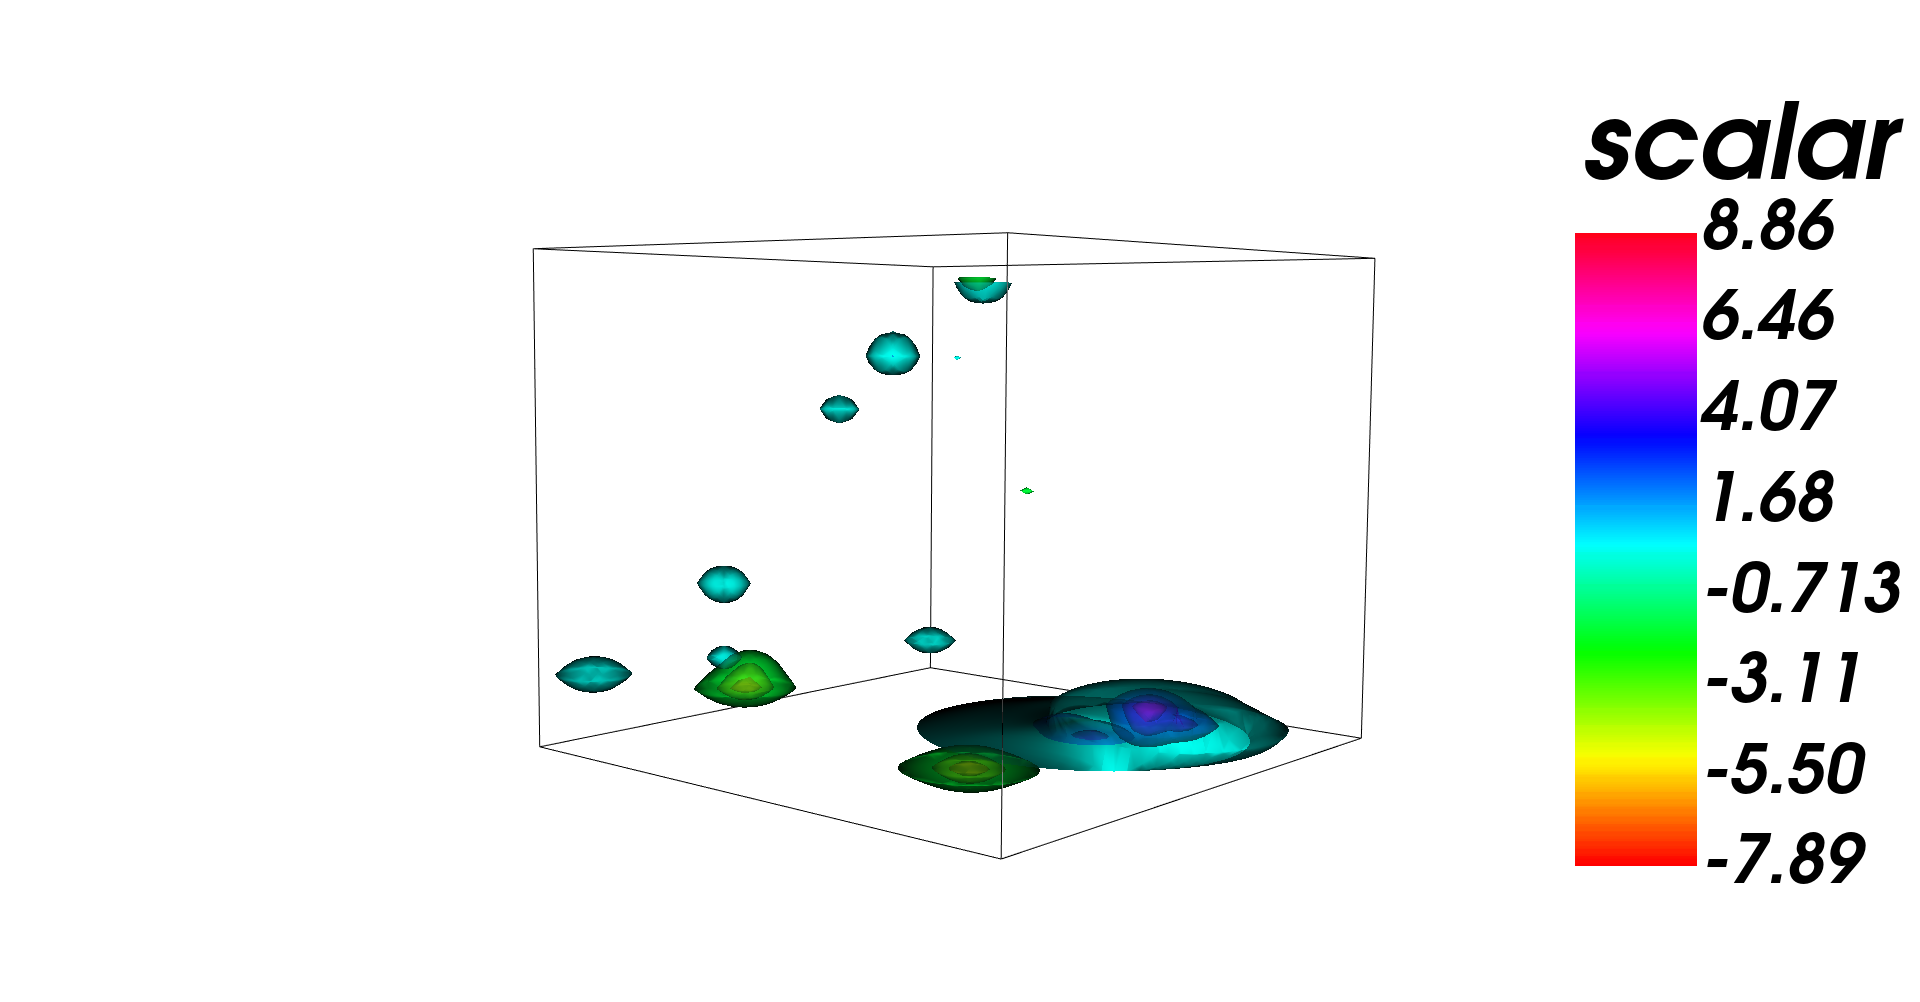
\includegraphics[width=0.7\textwidth]{snapshot.png}
\end{figure}
\end{frame}

\begin{frame}{Plans}
    \begin{Huge}
        Thanks !!
    \end{Huge}
\end{frame}

\end{document}

